\documentclass[review]{elsarticle}
\usepackage{graphicx,multirow,color,natbib,amssymb}
\journal{Tectonophysics}

\graphicspath{ {figures/} }

\newcommand{\cc}[1]{\textcolor{red}{#1}}

\begin{document}
\begin{frontmatter}

\title{Seismic parameter estimation and the Canadian crust}

\author[ubc]{B. Postlethwaite\corref{cor1}}
\ead{bpostlet@eos.ubc.ca}
\author[ubc]{M. G. Bostock}
\ead{bostock@eos.ubc.ca}
\author[ubc]{N. I. Christensen}
\author[gsc]{D. B. Snyder}

\cortext[cor2]{Corresponding author}

\address[ubc]{Earth and Ocean Sciences, UBC, Vancouver BC, Canada}
\address[gsc]{Geological Survey Canada, Natural Resources Canada, Ottawa ON, Canada}
%% ------------------------------------------------------------------------ %%
\begin{abstract}
It has been suggested that processes driving crustal formation in the Archean and Proterozoic were dissimilar and produced crusts with unique bulk properties and average thicknesses. The calibration of models based on evolving mantle fractionation or mantle convection style require accurate estimates of the geological and geophysical properties of crustal provinces to better constrain the details of crustal formation. Fifteen years of publicly accessible teleseismic data from all available Canadian seismic stations are binned in horizontal slowness and deconvolved into receiver functions. We apply a stacking method to retrieve estimates of the bulk crustal velocity ratio $V_P/V_S$ and thickness $H$ from these data under the assumption of locally 1-D structure. We also investigate modifications to this approach that can allow discrimination of $V_S$ and $V_P$ under certain conditions. Bootstrap error analysis is performed for each station dataset and subsets of these measurments are compared with results for matching stations from previous studies. Analysis of results in conjunction with additonal velocity estimates from active source seismic studies and a seismic property database affords improved constraints on bulk geological composition of the Canadian landmass that are used to evaluate competing models of crustal formation.
\end{abstract}

\end{frontmatter}
%% -----------------------------------------------%%
\section{Introduction}

The Canadian continental lithosphere is composed of at least fifteen large geological provinces representing crustal evolution from the early Archean to the present accretionary growth and orogenic deformation in the Western Cordillera. The Precambrian Canadian Shield and the bounding platforms of North America's interior comprise the cratonic core of Laurentia (Hammer et al., 2010). Several distinct geological provinces brought together during a series of Paleoproterozoic orogens make up the Canadian Shield (Hoffman, 1988, Figure 1). The largest of these provinces, and the world's largest Archean craton, is the Superior Province. Bounded by Proterozoic orogenic belts, the western and sourthern Superior is composed of roughly east-west trending geological subprovinces that include the granite-greenstone terranes of the Abitibi Greenstone Belt, metasedimentary gneisses, high-grade gneisses and plutonic complexes assembled during the period between 3-2.6Ga (Thurston et al., 1991). In the northwest of the Superior Province on the eastern shores of the Hudson Bay lies the Nuvvuagittuq greenstone belt that recent geochronological work has dated at ~4.28 Ga making it the only known remnant of Hadean crust preserved on Earth (O'Neil et al., 2011). To the east lies the younger, 1.2-0.98Ga, Grenville orogen, consisting largely of Superior and Southern Province rock reworked during Alpine-Himalayan like continental collision (Eaton et al., 2006). North of the Superior Province and separated by the Paleoproterozoic Trans-Hudson Orogen are the Rae and Hearne domains which together form the western extent of the Churchill Province. Studies of the the Rae suggest a Paleoarchean and Mesoarchean basement whereas the Hearne comprises granite-and-greenstone terranes of ages ~2.7Ga (Thompson et al., 2010). The Slave Province is a relatively small Archean granite-greenstone block lying to the northwest of the Churchill province. Its western portion is the 4.0 Ga remnant of a larger Archean continent, whereas the eastern Slave forms a younger (2.6 Ga) paired accretionary prism and island arc (Kusky, 1989). To the west of the Superior is the extensive Interior Platform overlying the southern extensions of the Trans-Hudson Orogen, Hearne Domain and Alberta Orogen. The Interior Platform is largely Archean reworked during the Paleoproterozoic with bore-hole samples indicating amphibolite to granulite-grade Proterozoic metamorphism (Hammer et al., 2010). Extending west from the Interior platform, the Western Cordillera developed in a passive margin setting on and adjacent to late Archean to Paleoproterozoic crystalline basement. Between the middle of the Jurassic and Paleocene intense metamorphic, plutonic and uplifting events occured as the result of Paleozoic and younger intraoceanic-arc accretionary events. The Coast Mountains evolved during the late Cretaceous as a wide magmatic arc composed largely of granitic rock (Clowes et al, 1995). Although there is considerable variation in structure and tectonic history, roughly half of the Cordillera is underlain by Proterozoic-margin crust that forms a crustal-scale décollement beneath interleaved and duplexed crust (Hammer et al., 2010). The rich tectonic tapestry of the Canadian continental crust affords an excellent opportunity to study variations in bulk crustal properties with geological age.

Our knowledge of the continental crust in Canada, in particular its thickness and structure in depth, has advanced greatly through Lithoprobe, a now complete national geoscience project spearheaded by active-source seismic profiling (Clowes et al., 1999). The full suite of Lithoprobe seismic profiles form a near-continuous transect from the Pacific to the Atlantic Oceans, and has enabled many insights into crustal structure and genesis. Recent summary studies utilizing Lithoprobe data include the analysis of Eaton (2005) who considers seismic observations in light of several hypotheses for the origin of the continental Moho: relic Moho, underplating, metamorphic front and regional d\'ecollement. Seismic evidence of preserved island arc Moho in Cascadia supports the first hypothesis whereas the presence of high-velocity, lower-crustal xenoliths in southern Alberta favours thick mafic underplating. Eclogite mineral assemblages forming a deep crustal root below the Grenville Front lends support to the third hypothesis, that at least in some places, continental Moho forms by large-scale eclogitization of the lower crust. Finally, seismic imaging of subhorizontal reflections separated by dipping reflection fabrics beneath the southern Canadian Cordillera suggests decoupling of the upper crust from the mantle during deformation and is taken as evidence for the fourth hypothesis, that an overprinted Moho may serve as a subhorizontal regional d\'ecollement. A subsequent study by Cook et al. (2009) argues that the continental Moho has varied and complex origins and that its imprint evolves through the effects of temperature, pressure, deformation and fluid migration.

In another recent summary study of Lithoprobe data, Hammer and Clowes (2011) discuss broad structural characteristics of the Canadian crust and note that Archean cratons and their boundaries contain structures similar to those found in Proterozoic and Phanerozoic orogens. They also discuss the lack of evidence for significant crustal disruption from magmatic instrusion related to subduction, post-orogenic extension or orogenic collapse. The authors remark upon the striking uniformity in Moho depth that is imaged between 33km and 43km depth along 20,000 km of Lithoprobe transects, despite the diversity of overlying crust. Both Cook et al. (2009) and Hammer and Clowes (2011) raise the possibility that, in some circumstances, the Moho and the base of seismic reflectivity do not represent the petrological crust-mantle boundary but rather eclogitized lower crust that is seismically indistguishable from the upper mantle. If this is the case, the seismic Moho would represent the top of a metamorphic front and would be shallower than the crust-mantle boundary.

The Lith5.0 revised crustal model presented by Perry, Eaton and Forte (2002) was developed from crustal thickness estimates taken from Lithoprobe seismic profiles. This work updates the global Crust5.1 model (Mooney et al, 1998) and introduces broad crustal features of the Canadian crust such as relatively thin Archean Shield regions (32.5-40.0 km) as compared to the thick ($>$42.5km) Phanerozoic crust in the south and west of the continental craton.

In this study, we examine the additional constraints that analyses of teleseismic receiver functions place upon Canadian bulk crustal properties when combined with available active source results. It is widely appreciated that receiver functions are sensitive primarily to crustal thickness and Poisson's ratio (or equivalently $V_P/V_S$) (Zhu and Kanomori, 2000), and that the latter quantity provides some ability to discriminate among possible bulk compositions (Zandt and Ammon, 1995). The constraint on Poisson's ratio and the greater averaging performed by low frequency (0.04-3 Hz) scattered teleseismic waves versus high frequency (10-40 Hz) {\it P}-waves employed in active source studies render the two techniques somewhat complementary. Our data set comprises the majority of teleseismic data available for the Canadian landmass including both permanent and temporary deployments. Many of the temporary deployments are described in (Bostock et al, 2010). Three previous studies employing similar methodologies but with more regional emphases deserve special mention: an examination of crustal thickness and $V_P/V_S$ variation in the Grenville Orogen (Eaton et al., 2005), a structural and compositional characterization of the Superior Province (Darbyshire et al. 2006) and a crustal evolution analysis of the Hudson Bay region (Thompson et al., 2010). Results from these studies will serve as benchmarks for our expanded effort. In the following sections we describe the data and methods employed to interrogate the Canadian crust. We proceed to present the major results beginning with a comparison between our seismic parameter estimates and the estimates from three studies mentioned above for identical seismic stations. We then present the results of a modified approach to our parameter estimation method and follow this with a presentation of the resulting crustal property estimates.  First presented are the average crustal discontinuity and structural patterns across Canada. Second, we take a tour through those geological provinces for which sufficient data exists, focusing on regional variation and characterization. We conclude with a discussion on the implications for our understanding of the composition and evolution of the Canadian Crust.

%% -----------------------------------------------%%


\section{Data and methods}


\begin{figure}
  \centering
  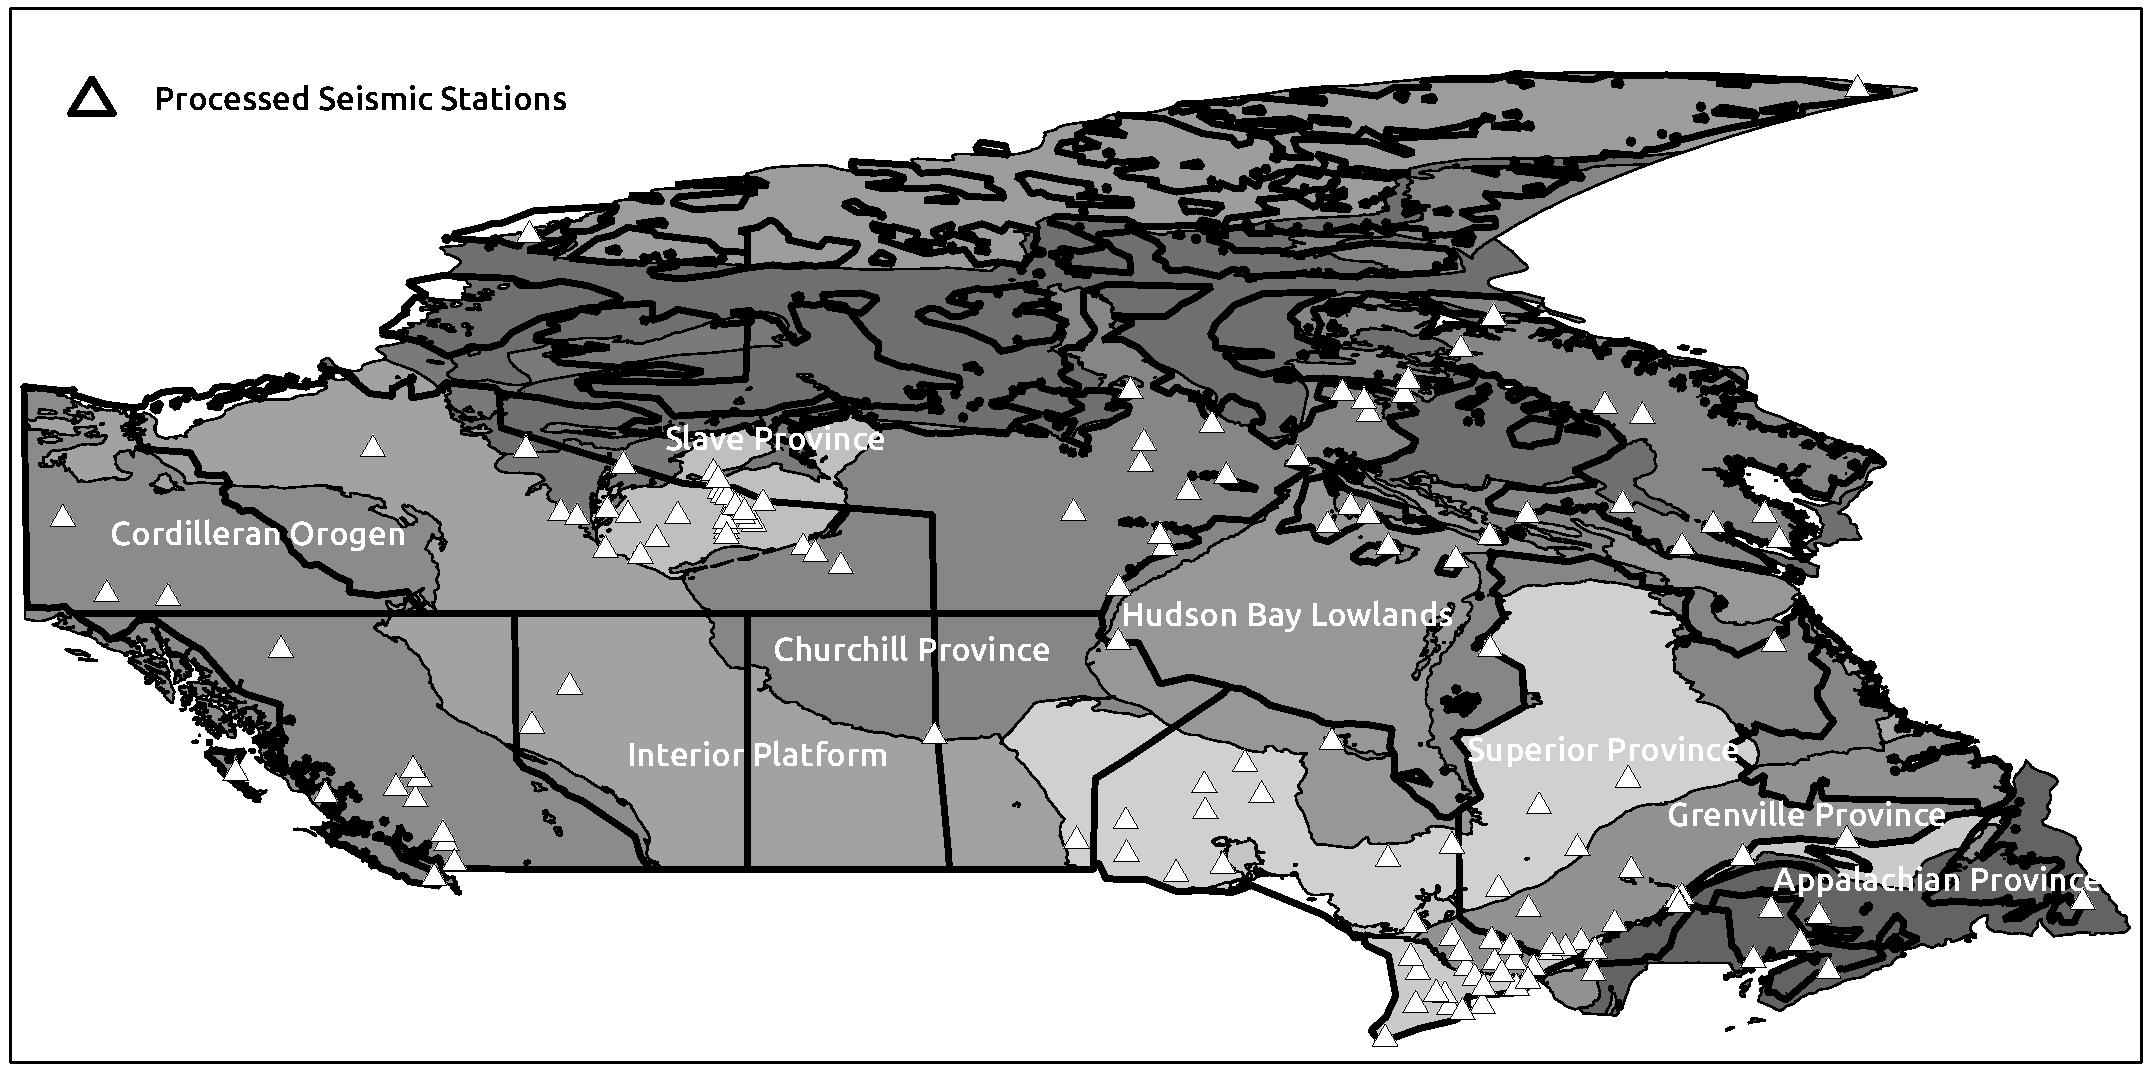
\includegraphics[width=\textwidth]{stationMap.pdf}
  \caption{Map showing major Canadian geological provinces and seismic stations contributing to the data discussed in this study.}
  \label{map:stationMap}
\end{figure}


Our analysis of bulk Canadian continental crust is based on estimates of crustal properties that can be accessed via seismic techniques, namely seismic wave velocities (or velocity ratio) and crustal thickness. This study draws on three sources for these crustal properties. The first and primary source is teleseismic receiver function (hereafter RF) analysis. The remaining two datasets are Crust 1.0, a widely published statistical average of similar regions with a global two degree resolution, and a compilation of pre-processed active source data (Mooney, 2012). Both Crust 1.0 and the active source compilation are used to qualify and compare with the primary dataset.




\subsection{Teleseismic Data Set}
The primary data utilized in this study are computed from teleseismic {\it P} wave seismograms originating from more than 700 earthquake sources. These earthquakes occurred between 2000 and 2012 and were recorded on subsets of 343 broadband seismic stations distributed across Canada. Seismic stations are selected from all available regional and national networks including CNSN, POLARIS, FedNor and Chasme. Seismograms are included for analysis if they fall within a 30 to 100$^\circ$ epicentral distance window. Quality control is performed by admitting only those seismograms with sufficiently high signal to noise ratios to permit visual observation of the dominant {\it P} wave energy and with sufficiently impulsive first arrivals to allow arrival onsets to be accurately measured. After selection and filtering more than 80,000 events are available for further processing. Seismic stations contributing to the data utilized in this study are shown in figure \ref{map:stationMap}.

The first stage of processing requires the transformation of teleseismic data into receiver functions. In general terms, this transformation involves deconvolving an approximation of the earthquake source from horizontal recordings of ground motion (Langston, 1979). The resulting waveforms contain discrete pulses corresponding to {\it S} waves scattered from subsurface discontinuities including the base of the crust, or Moho. Confident identification of these peaks is required to estimate crustal parameters, and improved results can be obtained by transforming the displacement seismogram into their {\it P} and {\it S} contributions based on a 1-D model of propagation. This procedure is accomplished by first rotating the N and E coordinates into radial and transverse directions and then performing a wave field decomposition using the radial and vertical channels (Kennet, 1991). The direct {\it P} arrival of the signal on the resulting {\it P} wave component is used as an approximation to the source function as {\it P} component impulse response for teleseismic P approximates a delta function. This windowed source estimate is deconvolved from the {\it S} wave component computed from the wave field decomposition.

We employ an $L_2$, multichannel, frequency domain approach to perform the deconvolution that has the advantage of computational efficiency and does not require {\it a priori} assumptions concerning the noise levels in the data. More specifically, we employ a simultaneous deconvolution of $N$ seismograms sharing a similar slowness to compute a single impulse response or receiver function $r(t)$.

% Deconvolution equations
\begin{equation}
  r(t) = {\cal F}^{-1} \left( G(\omega) \right) = {\cal F}^{-1}
 \left[ \frac {\sum_n^N S_n(\omega)P_n^*(\omega)} {\sum_n^N P_n(\omega)P_n^*(\omega) + \delta} \right ],
\end{equation}

\noindent where $F^{-1}$ is the inverse Fourier transform, $S_n$ represents the $n^{th}$ {\it S} wave seismogram, $P_n$ is the corresponding windowed {\it P} wave seismogram, $^*$ denotes complex conjugation and $\delta$ is the regularization parameter controlling the trade off between model smoothness and data misfit. The parameter $\delta$ which is chosen programatically by minimizing the general cross validation function $GCV(\delta)$ is given by

\begin{equation}
  GCV(\delta) = \frac {\sum_n^N\sum_m^M \left( S_n(\omega_m) - P_n(\omega_m)G(\omega_m) \right)^2 }
                      { \left( NM - \sum_m^M X(\omega_m) \right)^2 },
\end{equation}

\noindent where

\begin{equation}
  X(\omega_m) = \frac {\sum_n^N P_n(\omega_m)P_n^*(\omega_m)} {\sum_n^N P_n(\omega_m)P_n^*(\omega_m) + \delta},
\end{equation}

\noindent and $\omega$ is the frequency bin in the discrete Fourier transform. All resulting receiver functions, $r(t)$, are filtered between 0.04Hz and 3.0Hz.



\subsection{Vp/Vs method} \label{section:VpVsMethod}

\begin{figure}
  \centering
    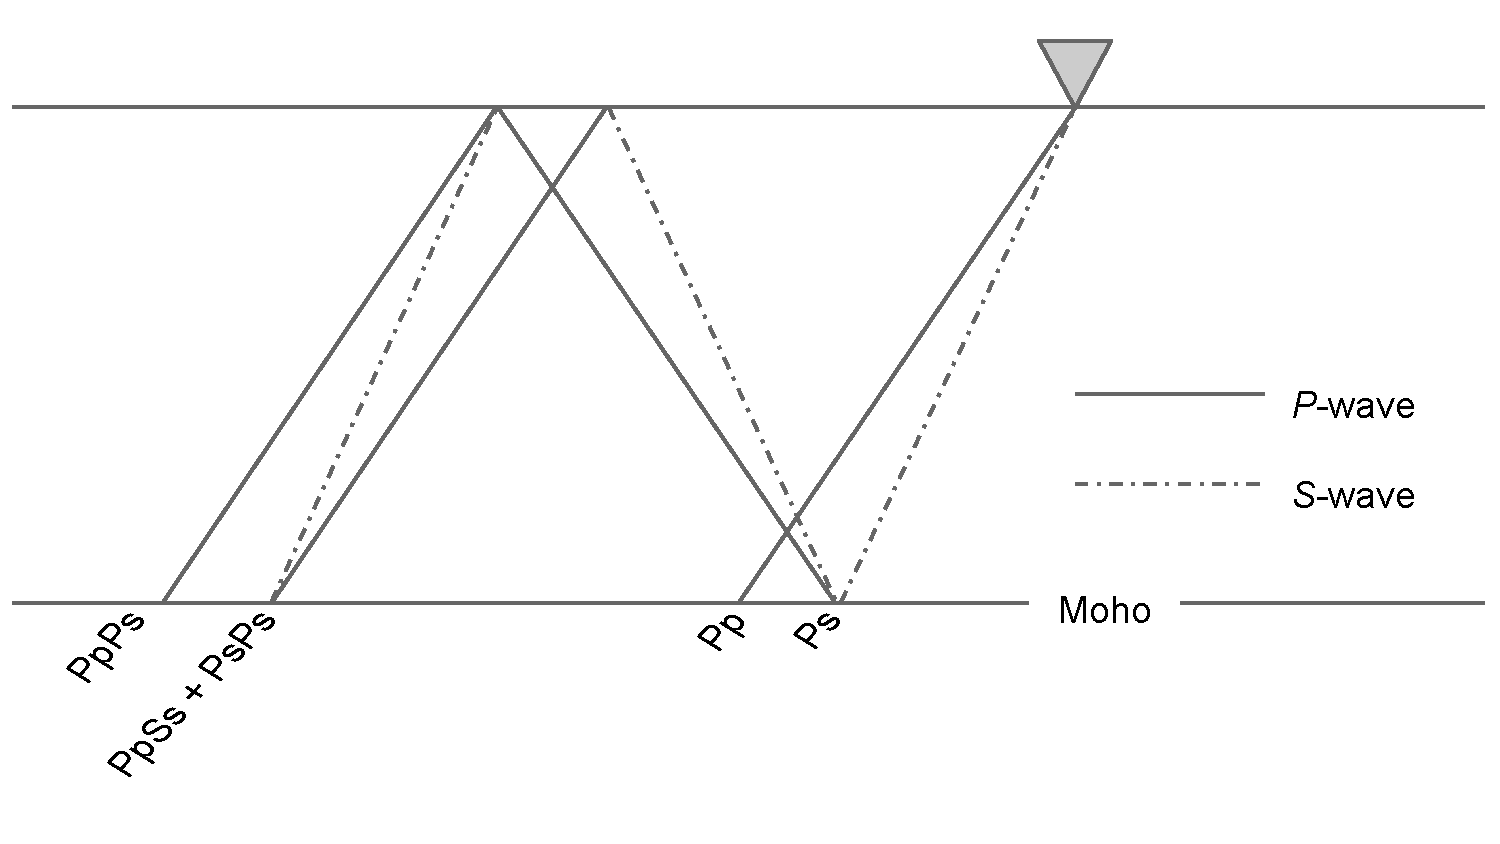
\includegraphics[width=\textwidth]{reflectedPhases.pdf}
  \caption{Schematic diagram illustrating geometry of phases for the velocity contrast representing the Moho}
  \label{fig:reflectedPhases}
\end{figure}


A well tested and widely published method for extracting the ratio of {\it P} velocity $V_P$ to {\it S} velocity $V_S$, herafter referred to as $R$, and crustal thickness (or depth to Moho) $H$, is outlined by Zhu and Kanamori (2000), hereafter ZK. This method exploits the dependence of these parameters to the differential arrival times between the {\it S} wave reflected phases $Ps$, $PpPs$, $PsPs$, $PpSs$ and $PsSs$ and the direct {\it P} wave arrival $Pp$ (Fig \ref{fig:reflectedPhases}). Note that $PsPs$ and $PpSs$ are kinematic analogues, such that the energy for these two phases arrive simultaneously for a 1-D model. For a range of slowness values, $p$, the differential arrival times, $t(p)$, trace moveout curves for each phase arrival given by

% Travel time equations
\begin{equation} \label{eq:tps}
t_{Ps}(p_n) = \frac{H}{V_P} \left( \sqrt{ R^2 - V_P^2p_n^2} - \sqrt{1 - V_P^2p_n^2} \right)
\end{equation}

\begin{equation}
t_{Pps}(p_n) = \frac{H}{V_P} \left( \sqrt{ R^2 - V_P^2p_n^2} + \sqrt{1 - V_P^2p_n^2} \right)
\end{equation}

\begin{equation}
t_{Pss}(p_n)= \frac{2H}{V_P} \sqrt{ R^2 - V_P^2p_n^2}
\end{equation}

\noindent where $p_n$ is the slowness for the $n^{th}$ receiver function. Since strong reflected phases occur at sharp velocity contrasts, the Moho, the boundary targeted by ZK, tends to be well represented on most RF's.

The travel time equations, as employed by ZK, assume a value for crustal {\it P} wave velocity, $V_P$, that in practice will trade-off to some degree with crustal thickness $H$. In our implementation of the ZK approach, each station is assigned a $V_P$ value corresponding to the Crust 1.0 value for the corrisponding $2^\circ$ containing cell. In the specific cases where data are being compared to previously published results for quality control, $V_P$  values are chosen to match the values in the published study.

RFs are stacked along trial moveout curves for a range of candidate models of $R$ and $H$ to generate a fitness function $s(H,R)$.  Within the stacking procedure, each phase is assigned a weight to account for the expected relative amplitudes of the phases for typical velocity contrasts, with the direct conversion $Ps$ usually characterized by the highest quality signal followed by $PpPs$ and $PpSs$. We chose weights of $w1 = 0.5$, $w2 = 0.3$ , $w3 = -0.2$ for the $Ps$, $PpPs$ and $PpSs$ phases, respectively. A negative weight for the combined $PpSs$ and $PsPs$ phases is required as the polarity of the signal is reversed. Semblance weighting (Eaton, 2006) is employed to reduce the effect of spurious large amplitude noise in the data. The semblance function assigns a weight between zero (incoherent noise) and one (coherent signal). The stacking function is therefore defined as

\begin{equation}  \label{eq:stack}
s(H,R) = \sum_{m=1}^{3} S_m \sum_{n=1}^N w_mr_n(t_m)
\end{equation}

\noindent where

\begin{equation}
S_m(H,R) = \frac {\left( \sum_{n=1}^N r_n(t_m) \right)^2}
                 { \sum_{n=1}^N r_n^2(t_m) }
\end{equation}

\noindent is the semblance weight for the $m^{th}$ phase, time $t_m$ is calculated from the corresponding travel time function for a given $H$, $R$ pair as a function of slowness $p_n$ and $N$ is the total number of receiver functions. Multiplying by the semblance weighting sharpens the stacked image, $s(H,R)$, and results in better resolution when discriminating between different models. The function $s(H,R)$ can be thought of as a transformation that maps times of the $Ps$, $PpPs$ and $PpSs+PsPs$ phases into $R$ and $H$ space as positive bands, via Eq. \ref{eq:stack}. Constructive interference where these bands intersect produce a maximum in the stacking function. The model, $R$ and $H$, that produces this maximum provides the best estimate for the bulk crustal parameters for a given seismic station.

A limitation of the ZK approach is the requirement of an initial $V_P$ estimate. In principal we may compute the stacking function Eq. \ref{eq:stack}, as a function of all three seismic parameters, $s(H,R,V_P)$. Taking advantage of modern multi-core systems with reasonable quantities of data (fifty to a few hundred RFs) and a moderate search space ($n^3$ parameter candidates where $n \approx 150$) the computational time makes this method easily scalable to hundreds of stations. This ``fullgrid'' approach is analyzed to determine the viability of recovering $V_P$.

The trade-off between $V_P$ and $H$ (and other parameter combinations) and error resulting from data quality are quantified for both the full parameter search and ZK methods by bootstrap resampling (Efron and Tibshirani, 1986). An estimate for the error is calculated in a bootstrap resampling approach by taking the standard deviation of 1024 parameter estimates each produced with randomly selected RFs, with replacement.




\subsection{Additional data}

We supplement receiver function estimates of crustal properties with data from controlled source experiments collected and compiled from GSC (Geological Survey of Canada) references by Walter Mooney (personal communication, 2012). The active source data provide $V_P$ and a few $V_S$ estimates for hundreds of locations across Canada, many along transects that cross major geological boundaries, faults and discontinuities. Some of these data are located within reasonable ($<$100 km) proximity to seismic stations used in this study and can be used to compare with the $V_P$ and $V_S$ estimates resulting from the RF full gridsearch.

The Crust 1.0 model (Laske et. al., 2013) employs many of these same active source data to provide regular, complete coverage across all of Canada. The model includes estimates of $V_P$ and $V_S$ information with depth at $1^\circ$ resolution in latitude and longitude. In addition to employing local active source data, Crust 1.0 is also constrained by statistically aggregated data from geographically distant but geologically similar regions. It therefore affords a somewhat independent dataset suited for comparison with the crustal estimates calculated in this study.

%% -----------------------------------------------%%

\section{Results}


\subsection{Comparisons}

Three published studies have provided parameter estimates for $R$ and $H$ for subsets of the seismic stations considered here. The most recent study (Thompson et. al., 2010) focused on the northern Canadian Shield and employs both the linear stacking approach used by ZK as well as a phase weighted method. A 2007 study of the Superior Province (Darbyshire et. al, 2007) and a study of the Grenville Orogen (Eaton et. al., 2006) utilize the ZK + semblance approach outlined in section \ref{section:VpVsMethod}.  Comparisons between crustal estimates of $R$ for particular seismic stations are made for those values with corresponding standard errors of less than $\pm$0.06. This error threshold is chosen empirically as that which best partitions those receiver function stacks with visually recognizable energy along phase moveout curves from those where lack of data or poor quality make these moveout curves difficult to distinguish. For each study under comparison, data are reprocessed using the $V_P$ chosen by the study authors. For the 2006 and 2007 studies the ZK + semblance method is used whereas for the Thompson et. al study the linear stacking ZK approach is employed. Both correlation coefficient and mean difference are provided in (Table \ref{table:comparison}) as measures of similarity.

\begin{table}
  \begin{tabular}{ p{3cm} p{2cm} p{1cm} p{0.5cm} p{0.5cm} p{0.5cm} p{0.5cm}}
    & & & \multicolumn{2}{ c }{Corr. Coeff.} & \multicolumn{2}{ c }{RMS difference} \\
    \hline
    Study Authors & Region & Num. Stns &  $H$ & $R$  &$H$ (km)& $R$ \\
    \hline
    Thompson et. al. (2010) & N. Canadian Shield & 29 & 0.97 & 0.70 & 0.78 & 0.017 \\
    Darbyshire et. al. (2007) & Superior Province & 10 & 0.95 & 0.43 & 1.71 & 0.037 \\
    Eaton et. al. (2006) & Grenville Orogen & 26 & 0.90 & 0.61 & 1.03 & 0.033 \\
    \hline
  \end{tabular}
  \caption{Comparison of $R$ and $H$ estimates with three published studies}
\label{table:comparison}

\end{table}

All three studies reported $H$ estimates that correlate strongly with the crustal thickness parameters computed here. The data from the northern Canadian Shield shows strong correlation in both $H$ and $R$. The lower correlation observed in estimates of $R$ than $H$ is not unexpected as the range of $R$ is relatively narrow and small changes ($\approx 2\%$) are physically meaningful. A corollary of this is greater sensitivity of $R$ to differences in procedure such as the choice of deconvolution algorithm and selection and scaling of data. The results from Thompson et. al. (2010) also corrispond most closely to the parameter estimates computed here, with the mean difference for both parameters being less than half of the averaged bootstrap error computed in this study. Results published by {\it Eaton et. al.} (2006) show reasonable correlations in both $R$ and $H$ and a mean difference for both parameters that is roughly equal to the averaged uncertainty in the data. Parameter estimates from the Superior Province (Darbyshire et. al., 2007) show the lowest correlation in $R$ as well as the highest mean difference in both parameters. These differences are well over the averaged computed error, and can not be easily explained by deviation related to noise in the data.

\subsection{Full Grid Search Analysis}

We now proceed to compare our results computed using the ZK approach with those from the full grid search. We note that the velocity ratio $R$ has a correlation between the two datasets of 0.76 whereas $H$ has a correlation of 0.51. The low correlation between crustal thickness estimates can be explained by the strong tradeoff between $H$ and $V_P$ through the quantity

$$\frac{t_{Pps}-t_{Ps}}{2}=\frac{t_{Pss}}{2} - t_{Ps}= \frac{H}{V_P}\sqrt{1-p^2V^2_P)}.$$

\noindent As a consequence, contours of the misfit surface $s(H,R,V_P)$ are highly extended along the kinematic curve in the $H$ - $V_P$ space (Figure \ref{fig:kcurves} a). This trade-off contributes to the low correlation in $H$ between the two methods. Higher correlation in this quantity (0.96) can be restored by dividing out $V_P$ from $H$. The trade-off between the other parameters is lower as there is greater dependence between them such that a small change in one necessitates a large change in an other to maintain travel-time equality, which has the result of a well defined misfit surface (Figure \ref{fig:kcurves} b-f).

For all but the cleanest stations, the trade-off between $H$ and $V_P$ renders recovery of $V_P$ unfeasible using the full grid approach. A comparison between two stations, ULM, the station with the highest quality RFs, and DORN, a station exhibiting less resolution in the reflected phases, illustrates this difficulty. RFs are arranged vertically, ordered by increasing slowness, and shown in figure \ref{fig:rfs}. Cross sections of $s(H,R,V_P)$ through each coordinate plane are displayed for ULM and DORN in figure \ref{fig:kcurves}. The lower resolution apparent in the $H$ - $V_P$ cross section for DORN translates into a bootstrap error of $V_P \pm 0.64 {\rm km/s}$. Station ULM, with cleaner data, has less trade-off between $H$ and $V_P$ as indicated by the corresponding cross section and the lower bootstrap error of $V_P \pm 0.16 {\rm km/s}$.

Active source experiments located near broadband seismic stations provide independent crustal thickness and {\it P} wave velocity estimates to test against data derived from the full parameter search method. We select stations with low error in $V_P$ and active source experiment locations within a 100 km radius. If several active source experiments are located within this radius, estimates are averaged. Four stations (ARVN, TYNO, ULM and WHY) meet these criteria and the parameter estimates are presented in figure \ref{fig:vpactive}. Estimates computed from the full grid approach are roughly 0.25 km/s higher than the active source data. This difference is consistent across all four stations and is exemplified by a 99\% correlation, suggesting possible bias. However, the limited number of data means this bias is poorly constrained.

There is less correlation between the crustal thickness data, though this is largely attributed to an approximate 10 km difference between the ARVN estimates. The reason for this discrepancy is unknown though both the ZK method and and a published study (Thompson et. al., 2010) provide an estimate of near 41 km for ARVN, much nearer the full grid value of 42 km. Despite lower correlation the apparent bias towards higher values computed from teleseismic data is also maintained for $H$. A positive bias in one parameter will tend to bias the other, owing to the relationship between thickness, velocity and times of a scattered phase. For a constant $t_{ps}$ one may compute how much $H$ must change for a 0.25 km/s bias in $V_P$ (Zhu and Kanamori, 2000). Using an average of the parameter estimates from the two cleanest stations, ULM and WHY, $\delta H$ will be 1.3 km, this fits well with the actual bias in the values.


\begin{figure}
  \centering
  \includegraphics[width=\textwidth]{kinematicCurves.eps}
  \caption{}
  \label{fig:kcurves}
\end{figure}

\begin{figure}
  \centering
  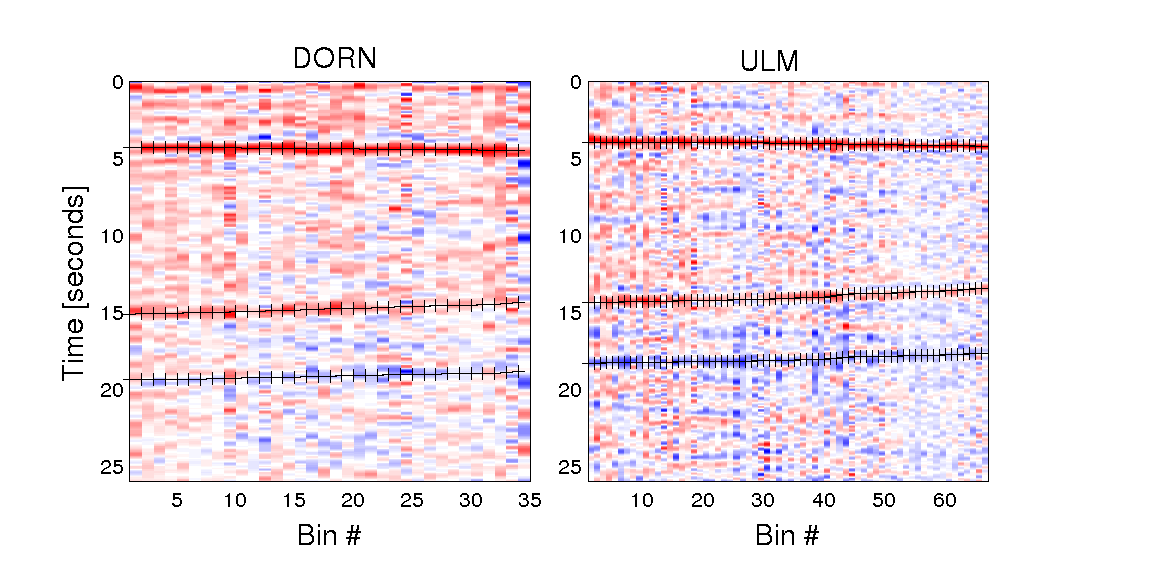
\includegraphics[width=\textwidth]{rfDORNULM.eps}
  \caption{}
  \label{fig:rfs}
\end{figure}


\begin{figure}
  \centering
  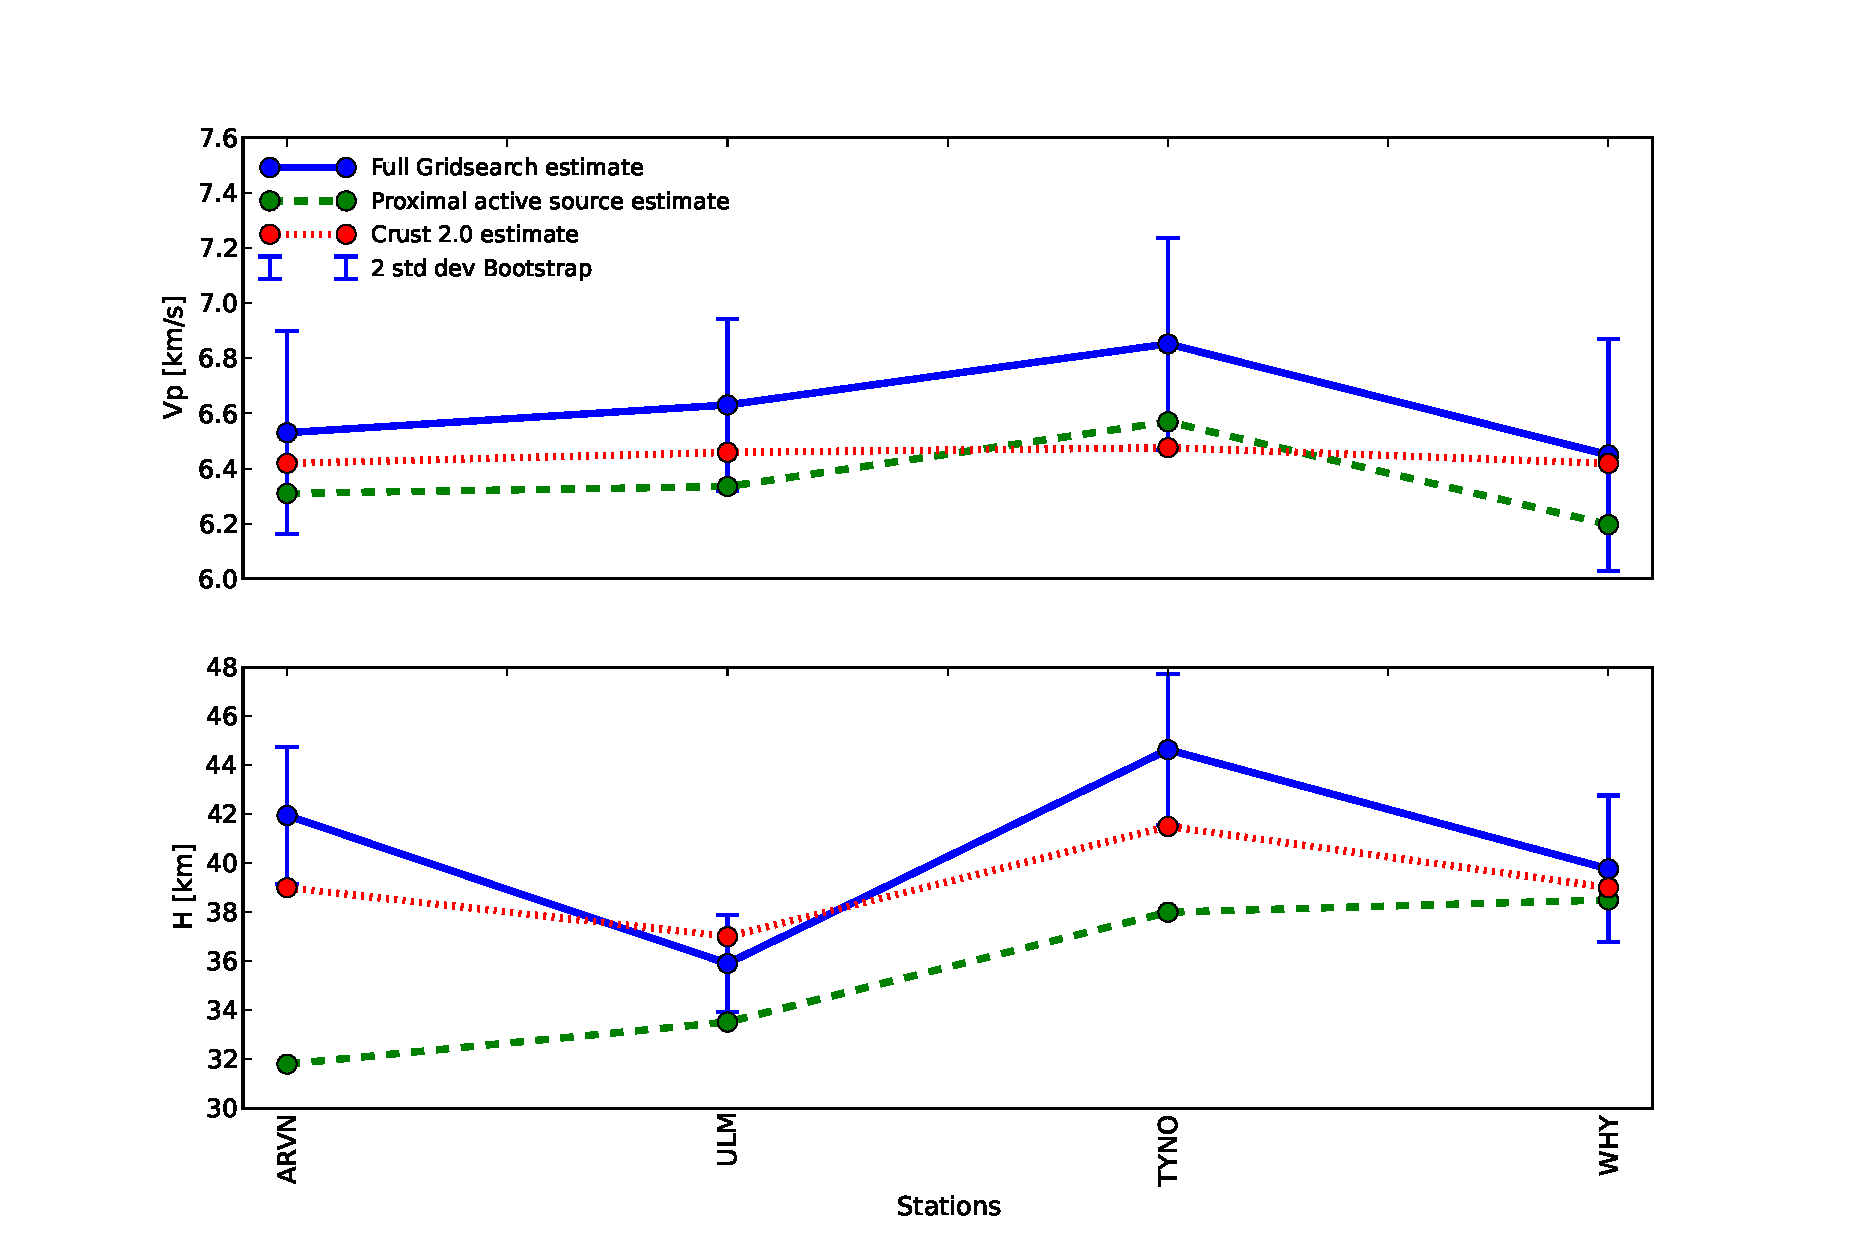
\includegraphics[width=\textwidth]{vpactive.eps}
  \caption{Top, {\it P} wave velocity estimates computed from the full parameter search method compared to active source data and values from Crust 1.0. Bottom, crustal thickness estimates computed from the full parameter search method compared to active source data and values from Crust 1.0}
  \label{fig:vpactive}
\end{figure}



\subsection{Crustal Discontinuities} \label{section:discontinuities}

\begin{figure}
  \centering
  \includegraphics[width=\textwidth]{discPCA.eps}
  \caption{Left, vertical station depth profiles. Right, the SVD singular vectors (principal components) of the station depth profile matrix. Each principal component represents a mode that captures some part of the total variance in the dataset. Vertical lines are the axis each profile and vector is normalized about. A grey horizontal window highlights a region of low energy.}
  \label{fig:discPCA}
\end{figure}

We now consider the average crustal structure across Canada. We produce a depth profile for each station by stacking receiver functions along traveltime curves corresponding to a range of values in $H$ (0 to 50 km in increments of 100 metres) using the estimates for $R$ computed via the ZK + semblance method. The resulting profiles contain energy at depths corresponding to major velocity discontinuities and are shown in figure \ref{fig:discPCA} (left) arranged by increasing crustal thickness. By assembling all depth profiles into a matrix, we may decompose the data via SVD into their principal components. Figure \ref{fig:discPCA} (right) contains the first five singular vectors or modes normalized to unit magnitude that account for 78\% of the variance in the profiles. Higher modes correspond to diminishing contributions to total variance. Each vector is normalized to unit magnitude. The first mode is effectively the average depth profile across all stations and captures 50\% of the variance in the dataset. It features a maximum near 38.7 km that may be taken as an average Moho depth. The second and third modes are dominated by a high amplitude shallow structures (e.g. sedimentary layers) within the top 10 km and Moho variability between 30 and 46 km . The fourth and fifth modes account for a combined 11\% of the variance in the dataset, contain energy at upper-mid crustal depths in the 10 km to 20 km range. All 5 modes display markedly lower energy within a depth window roughly between 20 km and 30 km.



\subsection{Regional Bulk Crustal Parameters}

We proceed to consider crustal thickness $H$ and velocity ratio, $R$, estimates for stations with assigned $R$ bootstrap errors below $\pm 0.06$ in a geographic context (figure \ref{map:stationMap}). To compensate for the uneven distribution of seismic stations, weights are applied to both $R$ and $H$ estimates before averaging over a given region. Weights are calculated by projecting station locations onto a 2D plane using the Albers equal-area conic projection. A Voronoi diagram is then computed using all projected station locations. The ratio between the Voronoi cell surface encompassing each station and the total area of the convex hull bounding region is employed as that station's weight.

Table \ref{table:regionParameters} displays the results of our regionalization in $R$ and $H$. The weighted average crustal thickness for all stations (Canada) is 37 km, about two kilometres thinner than the average for the Canadian Shield. Crust 1.0 provides a slightly thicker crustal average for Canada (38.1 km) and a slightly thinner average for the Shield (38.3 km). The Slave Province averages are similar to those for the Churchill province with a crustal thickness and seismic velocity ratio comparable to Crust 1.0. Moving south and east from the Churchill Province through the Superior Province into the Grenville Province, we note an increase in the ZK + semblance $R$ values as well as crustal thickness $H$. The weighted $R$ average is 1.73 in the Churchill Province increasing slightly to 1.74 in the Superior and jumping to 1.78 in the Grenville. In a similar fashion, the weighted average of $H$ increases from 38.9 km in the Churchill Province  to 39.7 in the Superior Province and 41.7 km in the Grenville Province. The southeastern trend towards increasing values is also expressed in weighted averaged active source $V_P$ data as well as as the Crust 1.0 $V_P$ data.  The Crust 1.0 model is characterized by slightly thinner crust though the southward thickening trend is noticeable. The trend in the seismic velocity ratio is not, however, as apparent.


\begin{table}
  \begin{tabular}{ l l l l l l l }
    \cline{2-7}
    & \multicolumn{2}{ c }{ZK + semblance} & \multicolumn{3}{ c }{Crust 1.0} & \multicolumn{1}{ c }{Active Source} \\
    \hline
    Region  & $H (km]$& $R$ &$H [km]$& $R$  &$V_P [km/s]$&$V_P [km/s)$ \\
    \hline
    Canada    & 37.0 & 1.75 & 38.1   & 1.74 &   6.41     & 6.33\\
    Shield    & 39.2 & 1.74 & 38.3   & 1.74 &   6.47     & 6.42\\
    Slave     & 38.2 & 1.74 & 38.0   & 1.73 &   6.47     & 6.44\\
    Churchill & 38.9 & 1.73 & 37.9   & 1.74 &   6.46     & 6.39\\
    Superior  & 39.7 & 1.74 & 38.9   & 1.74 &   6.49     & 6.44\\
    Grenville & 41.7 & 1.78 & 39.7   & 1.74 &   6.50     & 6.48\\
    \hline
  \end{tabular}
  \caption{Comparison of $R$ and $H$ estimates with three published studies}
\label{table:regionParameters}

\end{table}


%% -----------------------------------------------%%
\section{Discussion and Conclusions}

Seismic refraction and reflection studies of continental crust have afforded valuable constraints on the processes governing crustal evolution. Early efforts to characterize continental crust invoked a 2-layer, slab model comprising lower velocity upper crust and a higher velocity lower crust (Conrad, 1925; Jeffreys, 1926). Evidence supporting this model was originally presented by Conrad (1925) who cited observations of P arrivals propagating along a mid-crustal interface similar to but shallower than the deeper crust-mantle interface imaged by Andrija Mohorovičić in 1909 (Litak and Brown, 1989). Interpretations of seismic data invoking both the crustal slab model and the Conrad Discontinuity, as the mid-crustal interface became known, persisted in the literature but were increasingly criticized as being too simplistic, in the case of the slab model, or, for the Conrad Discontinuity, lacking consistent evidence (Litak and Brown, 1989). Technological improvements in reflection seismology allowed researchers to further argue for a complex heterogeneous crust and propose models wherein smooth random lateral inhomogeneities are superimposed on simple velocity gradient models to reproduce the range of seismic observations (Litak and Brown, 1989; Mereu and Ojo, 1981).

Despite diminishing support in recent years for the Conrad Discontinuity as a universal crustal feature, the division of the crust into seismically distinguishable upper and lower components remains a common assertion. In their review, Mooney and Brocher (1987) argued for a model of the continental crust separated into a seismically reflective lower crust overlain by transparent upper crust. Their physical interpretation is that of a poorly laminated upper crust dominated by features of short length scale that contrasts with a lower crust composed of thin ($\sim$ 100 m) lamellae of significantly longer horizontal length scale. The inference of a laminated lower crust has since found support in studies of regions with extended or thicker, warmer crust (e.g. Ito, 1998; Mayer, 1996; Meissner et. al., 2006).

\begin{figure}
 \centering
 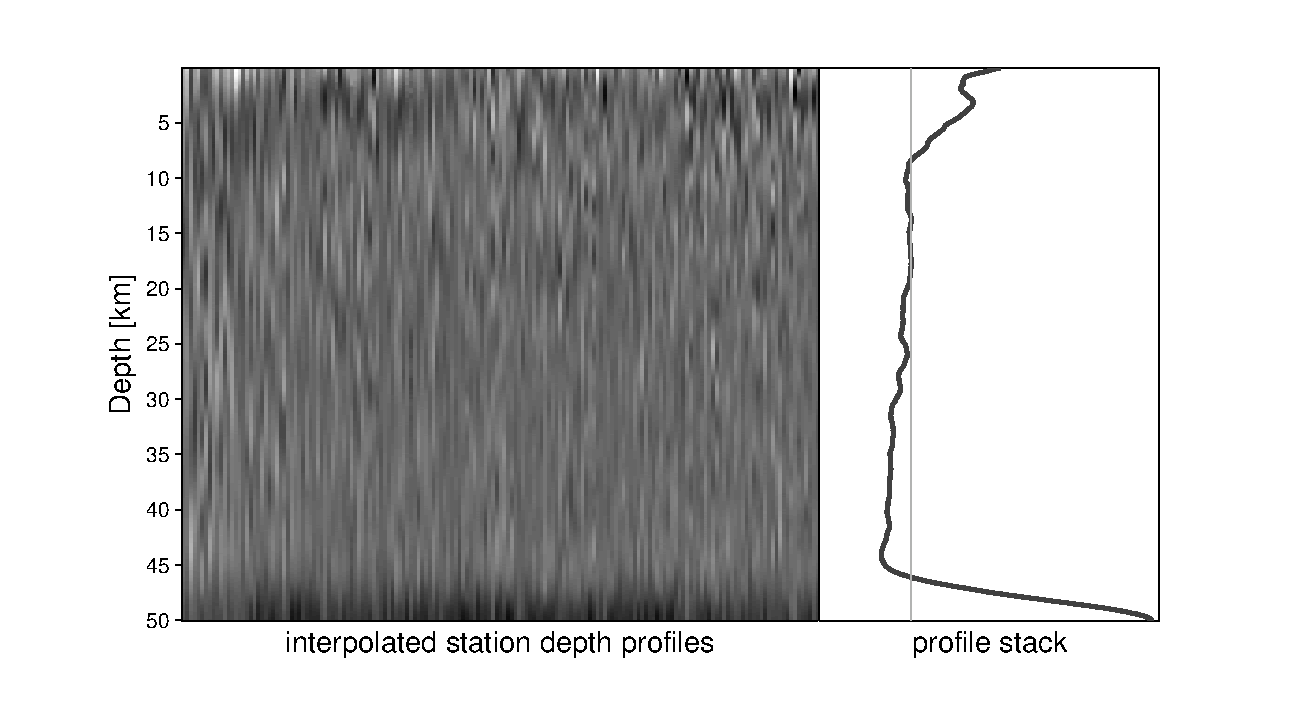
\includegraphics[width=\textwidth]{discInterp.eps}
 \caption{Left, vertical station depth profiles interpolated to a common Moho. Right, normalized stack of depth profiles, grey line shows mean}
 \label{fig:discInterp}
\end{figure}

The lower energy in the 20-30 km depth window noted in Section \ref{section:discontinuities} for the station profiles given in figure \ref{fig:discPCA} (left) provides some supporting evidence for seismically distinct upper and lower crustal layers. To better compare results across stations, we normalize each depth profile such that the Moho falls on a common ordinate (Figure \ref{fig:discInterp}, left) and stack the absolute values (Figure \ref{fig:discInterp}, right). The stacked signal has highest amplitude near the surface, where energy is associated with sedimentary layers, and at the Moho. There is a steady and marked decrease in energy over the bottom third of the profile that cannot be ascribed to sidelobe structure associated with the Moho pulse. This observation is ostensibly at odds with the Mooney and Brocher (1987) high reflectivity lower crustal model. Moreover, reflection profiles from {\sc Lithoprobe} transects (Hammer et. al., 2010) frequently display significant reflected energy through the crust with some transects including the Western Superior transect and the Cassiar in the Western Cordillera displaying pronounced reflectivity within the lower crust. We reconcile the teleseismic and active source observations of transparent versus reflective lower crust by considering the scale of vertical heterogeneity to which the methods are sensitive. Teleseismic body waves include both direct and reflected conversions that can originate from layering with velocity gradients over scale lengths of the order of $\lambda/2$ and $\lambda/4$, respectively, where $\lambda$ is the {\it P}-wavelength (Bostock, 1999). For 1 Hz teleseismic waves, crustal layering with scale lengths of 1000-2000 m should be resolvable. Higher frequency active source data (10-40 Hz) employing {\it P}-wave sources are sensitive to finer scale vertical structure with scales of 75-300 m. We infer then that the vertical scales of lower crustal reflectivity are limited to scale lengths under 100 m yielding a lower crustal structure that is relatively transparent to teleseismic waves but can yield strongly reflective signatures to near-vertical, active-source seismic profiling.  Some authors, for example Mayer et .al. (1996) in their study of the Rhine Graben, have employed the term Conrad discontinuity to refer to an interface or transition between transparent upper crust and reflective lower crust. It is possible in this context that the higher energy levels between 15 and 20 km on the 5th principal component in Figure 12, is a manifestation of such signals, but the lower energy levels ($<5\%$) in this mode would indicate that Conrad Discontinuity so-defined is at best weakly defined within the Canadian crust. This finding is supported by crustal models characterized by a first order continuously increasing velocity profile such as the gradual transition from a more silicic uppercrust to a more mafic lower crust in shields and platforms observed by Rolf Meisnner (Meisnner, 1986). It is also supported by the lack of evidence for a consistent mid-crustal reflection boundary in lithoprobe data (Hammer et. al., 2010). The increased transparency of the lower crust would appear to be better defined and relate to changes in rheology. Studies of crustal strength (Jackson, 2002) and deformation (Burov and Watts, 2006; Meisner and Rabbel, 2006) as well as the widely noted reduced seismicity of the lower crust indicate changes would support this contention; though see (Deichmann, 1991; Handy and Brun, 2004; Simpson, 1999) for competing evidence.

Mean crustal composition is another important parameter characterizing continental crust though it is important to distinguish it from actual lithological or mineralogical state of the crust. It serves as a representative, average quantity that affords constraint on crustal structure and evolution in space and time. Early attempts at estimating mean crustal composition were largely performed through extrapolations based on the surface sampling of upper crustal rocks (Rudnick and Gao, 2003). After the plate-tectonic revolution, Taylor (1967, 1977), proposed the `island arc' or `andesite' model which posited that bulk crustal chemical composition is equivalent to the average convergent-margin andesite. Several problems with this theory subsequently emerged; for example, average surficial island arc composition is more basaltic than andesitic and any crustal growth via basaltic basal accretion will only serve to magnify this compositional contrast. Hence this model cannot account for the intermediate composition of post-Archean crust. Recognition of these shortcomings led to the analysis of data from crustal refraction seismic surveys to interrogate middle and lower crustal levels and place constraints on their composition (Christensen and Mooney, 1995; Rudnick and Fountain, 1995). Unlike these latter studies, which also utilize surface and exposed upper-crust geological information, the present work adopts a bulk crustal seismic analysis along the lines of Smithson et. al. (1981) although, whereas Smithson utilizes mean crustal $V_P$, this study combines $V_P/V_S$ from teleseismic measurements with constraints on $V_P$ from previous active source studies as presented in the Crust 1.0 model.

\begin{figure}
  \centering
  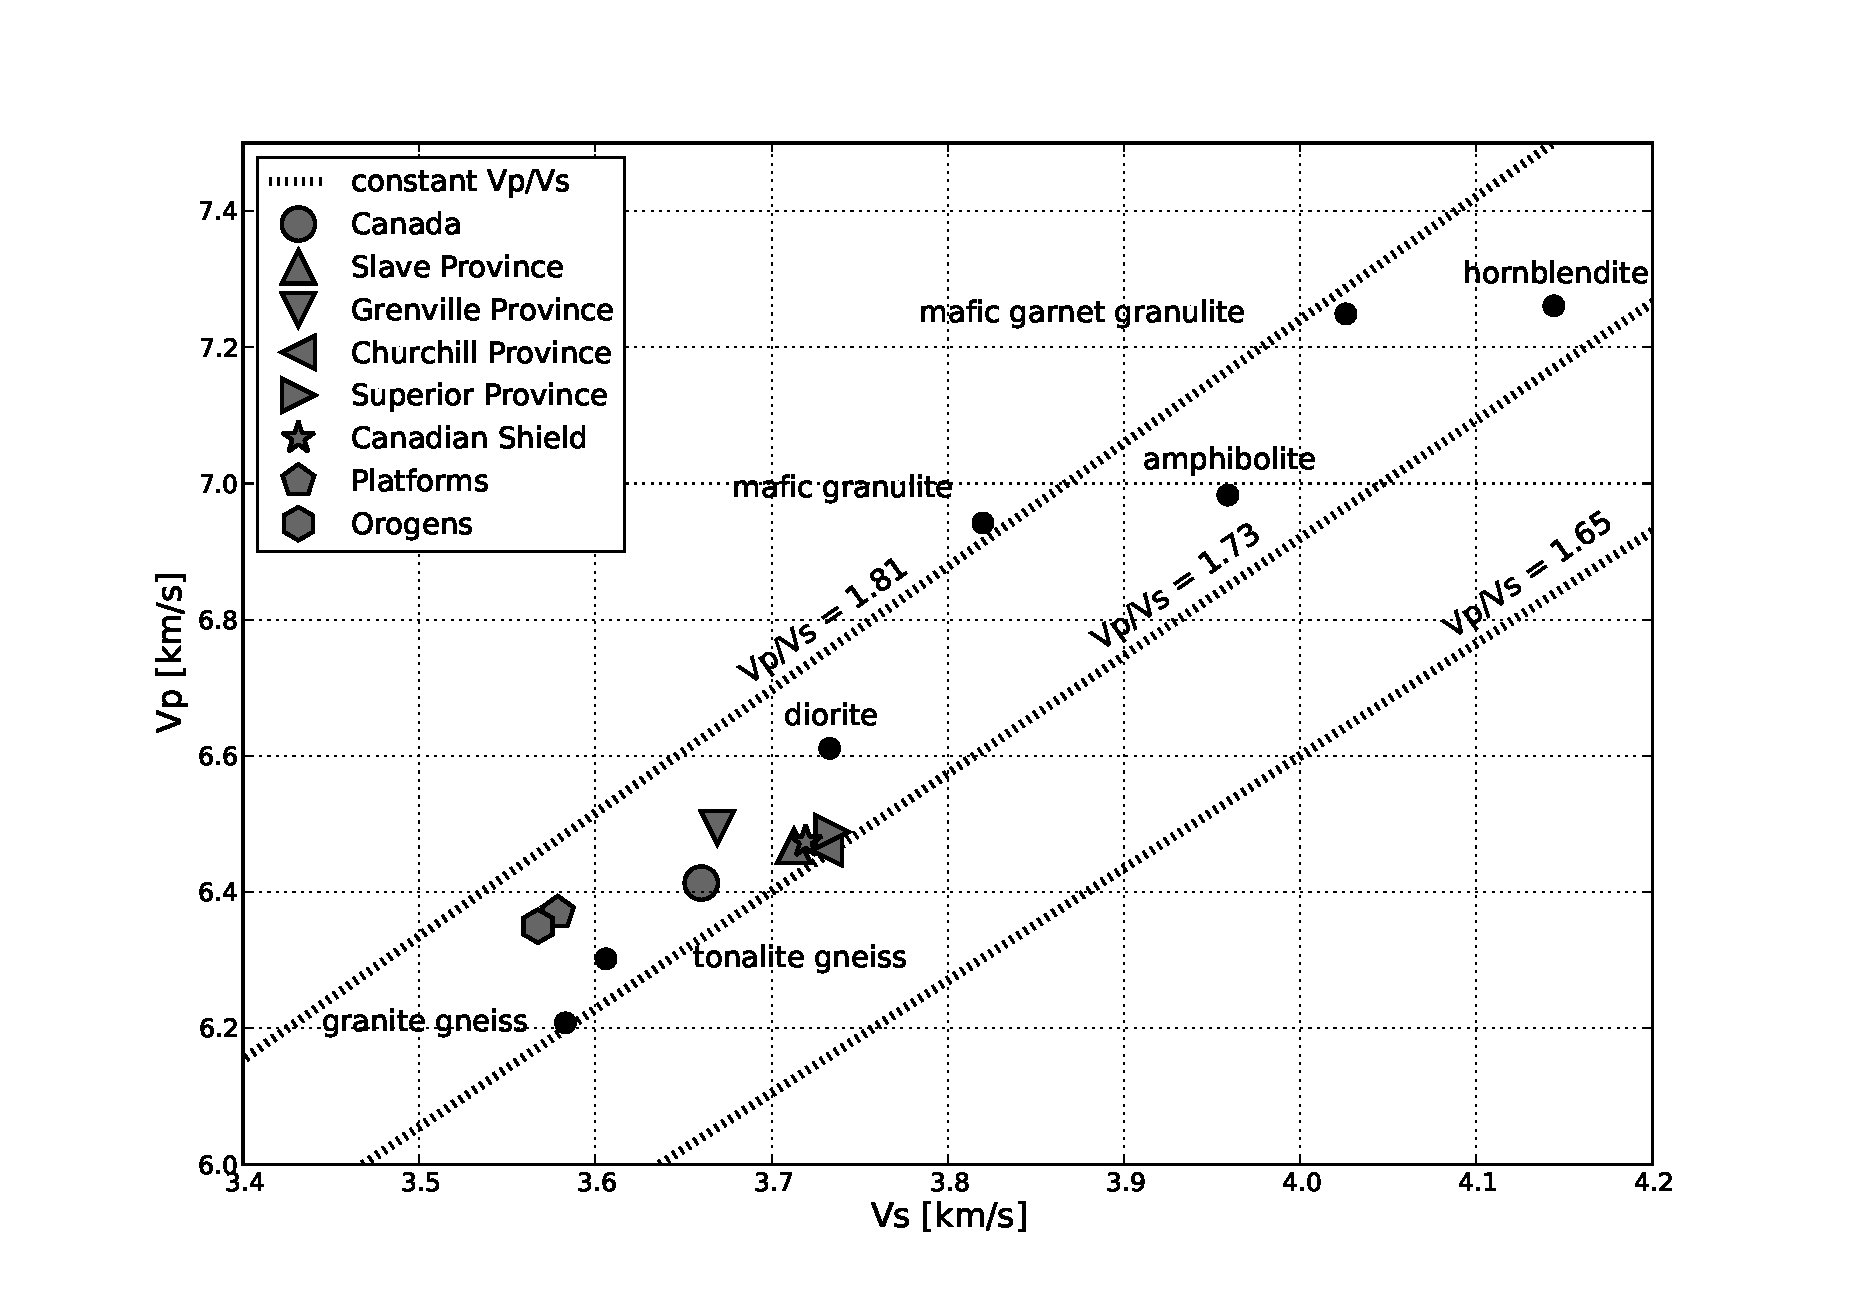
\includegraphics[width=\textwidth]{lithology.eps}
  \caption{$V_P$ and $V_S$ estimates for common crust lithologies and for major Canadian-Shield provinces}
  \label{fig:lith}
\end{figure}

In Figure \ref{fig:lith} we plot our area-weighted seismic parameter estimates for the entire Canadian data set along with area-weighted average estimates for various tectonic subdivisions on a graph of $V_P$ versus $V_S$. Also plotted are values for a selection of mineral assemblages considered to be representative of common crustal rocks from the compilation of laboratory measurements by Le Maitre (1976) and Christensen (1996), all quoted at average crustal pressures of 600 MPa. Dashed lines delimit isocontours in $V_P/V_S$. The choice of common shield lithologies is motivated by observations along 30km of paleo-depth represented in the Kapuskasing uplift of the Superior province (Percival and West, 1994). The Kapuskasing uplift comprises Archean granite-greenstone terranes dominated by granitoid and gneissic rocks, and contains supracrustal assemblages generally metamorphosed from greenschist to amphibolite and granulite facies and early plutonic structures comprised largely of tonalites and their metamorphosed equivalents. Tonalites and granodiorites are also part of the TTG (tonalite-trondhjemite-granodiorite) suite which dominates Archaean cratons (Rudnick, 1995).

Seismic parameter estimates for Canada and the Canadian Shield fall, to a first-order approximation, between those of two candidate end-member lithologies: granite geniss and diorite. This intermediate or andesitic composition is in general agreement with other earlier studies of bulk crustal composition e.g., (Rudnick and Fountain, 1995; Christensen and Mooney, 1995). The Slave, Superior and Churchill provinces possess comparable seismic parameters implying similar mean crustal compositions, with the Slave province represented as slightly more felsic in average composition. All three provinces cluster about the average value for the Canadian Shield. The Grenville Province, in contrast, displays markedly lower $V_S$ and higher $V_P/V_S$ implying a significant difference in mean composition. The high $V_P/V_S$ estimate, 1.77, is similar to the averaged results from a previous seismic study (Eaton et. al., 2005) that included stations of the central Grenville Orogen, and might be interpreted to indicate that the Grenville province possesses a mean crustal composition corresponding composition that is more mafic than other Shield provinces. This interpretation is consistent with a tectonic model for the the central Grenville Province which suggests that the mid-crust has been completely excised locally (Eaton et. al., 2005; Rivers, 2008). However, many stations in the south-east of the province also display $V_P/V_S$ ratios greater than 1.78, similar to the high values common in the adjacent St. Lawrence Platform (where the geometric mean seismic ratio is 1.79). Moreover, and more importantly, the average $V_P$ value for the Grenville province (a region well sampled by refraction profiles) requires low $V_S$ values that are inconsistent with a more mafic composition. Alternative explanations that allow for both high $V_P/V_S$ and reduced $V_P$, $V_S$ include the possibility that Grenville crust contains higher fluid concentrations than that of other tectonic provinces.


\begin{table}
  \begin{tabular}{ p{1.4cm} p{1.4cm} p{1.4cm} p{1.4cm} p{1.4cm} p{1.4cm} p{1.4cm}}
    \hline
    Oxide, wt\% & Pakiser et al. (1966) & Smithson (1978) & Christensen et al. (1995) & Rudnick et al. (2003) & This Work: Canada & This Work: Shield\\
    \hline
    $SiO_2$ & 57.9 & 63.0 & 61.7 & 60.6 & 64.3 & 61.9 \\
    $TiO_2$ & 1.2 & 0.7 & 0.9 & 0.7 & 0.6 & 0.7 \\
    $Al_2O_3$ & 15.2 & 15.8 & 14.7 & 15.9 & 15.5 & 15.9 \\
    $Fe_2O_3$ & 2.3 & 2.0 & 1.9 & --- & 1.9 & 2.1 \\
    $FeO$ & 5.5 & 3.4 & 5.1 & 6.7 & 3.3 & 3.9 \\
    $MnO$ & 0.2 & 0.1 & 0.1 & 0.1 & 0.1 & 0.1 \\
    $MgO$ & 5.3 & 2.8 & 3.1 & 4.7 & 2.2 & 2.8 \\
    $CaO$ & 7.1 & 4.6 & 5.7 & 6.4 & 4.3 & 5.1 \\
    $Na_2O$ & 3.0 & 4.0 & 3.6 & 3.1 & 3.6 & 3.6 \\
    $K_2O$ & 2.1 & 2.7 & 2.1 & 1.8 & 2.9 & 2.5 \\
    $P_2O_5$ & 0.3 & --- & 0.2 & 0.1 & 0.2 & 0.2 \\
    \hline
  \end{tabular}
  \caption{Bulk crustal composition comparison from selected sources. Rudnick and Gao (2003) use total $Fe$ expressed as $FeO$.}
\label{table:composition}

\end{table}

\begin{figure}
  \centering
  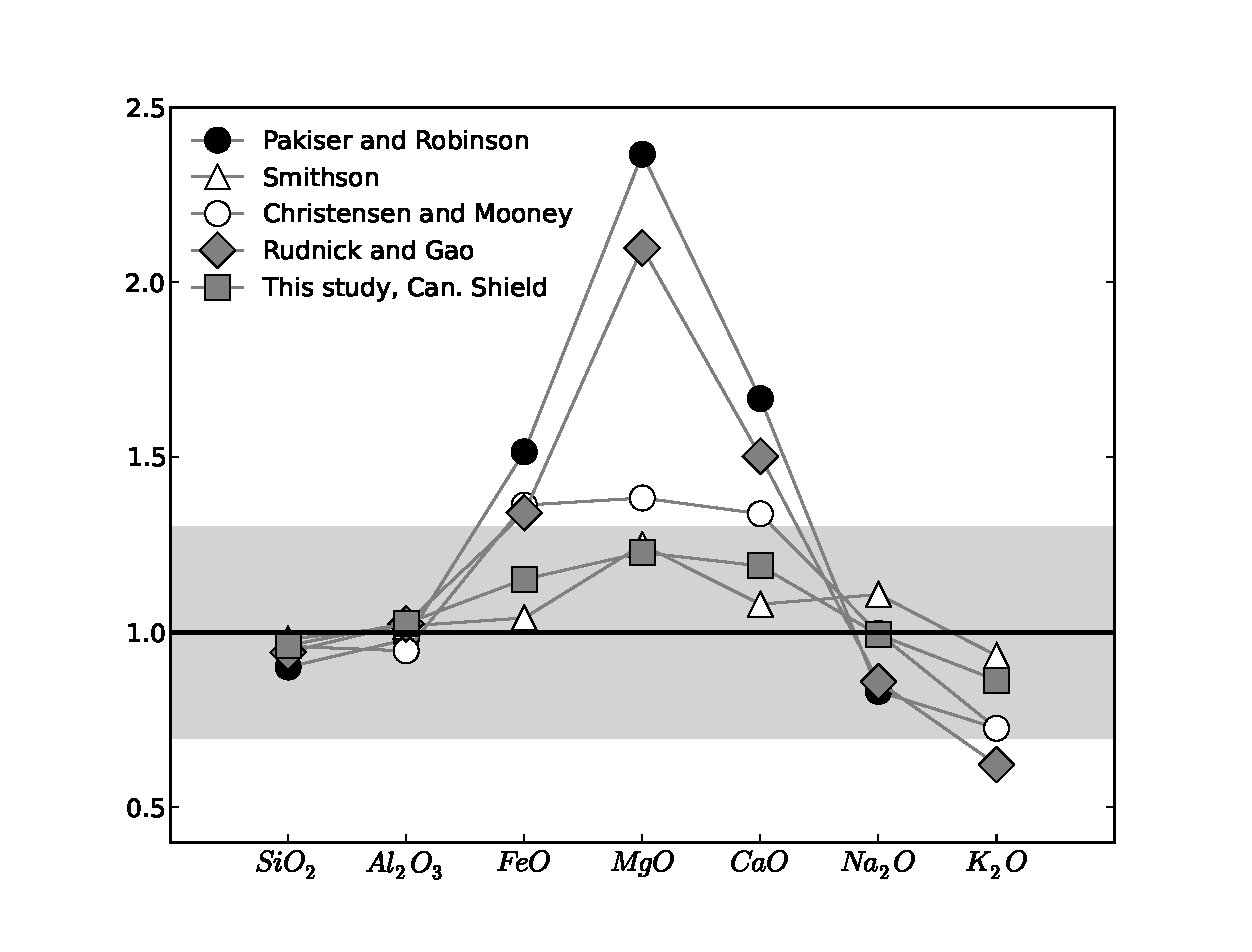
\includegraphics[width=\textwidth]{composition.eps}
  \caption{Comparison of major crustal elements from different studies. All estimates have been normalized to the results computed in this study.}
  \label{fig:composition}
\end{figure}

Since our average seismic parameter estimates for the entire Canadian crust lie on a line connecting diorite with granite gneiss (\ref{fig:lith}), we may estimate bulk crustal composition in proportion to these lithologies as 51\% diorite and 49\% granite. A similar estimate for the Canadian Shield is 68\% diorite and 32\% granite. This lithological ratio is applied to the chemical compositions of diorite and granite using chemical averages calculated from 141 diorite and 197 granite samples compiled by Le Maitre (1976) to produce an estimate of bulk crustal composition. The resulting chemical breakdown is provided in table \ref{table:composition} along with previous estimates from global crustal studies. Our analysis reveals a crust with marginally higher average $SiO_2$ composition and lower $MgO$ content than these previous studies. Figure \ref{fig:composition} displays the major crustal element contributions from the data in table \ref{table:composition} normalized to our average Canadian crustal composition. The gray-shaded region indicates the $\pm 30\%$ range from our reference average Canadian crustal model.  Also included in this figure is our average crustal composition estimate for the Canadian Shield. Its values closely track the global crustal estimates of Christensen \& Mooney (1995) and Smithson (1978). These data imply that the extensive platform and orogenic regions of Canada skew the average composition away from the global estimates of previous studies through incorporation of a higher proportion of granite gneiss. In contrast, the Canadian Shield crust aligns more closely with these previous global estimates.

Other researchers have employed Poisson's ratio (Zandt and Ammon, 1995) alone as an indicator of bulk crustal composition, and crustal thickness and {\it P}-wave velocity (Durrheim and Mooney, 1991) to constrain models of crustal formation. Zandt and Ammon (1995) report high $V_P/V_S$ values for Archean Shields and concluded that no systematic difference between Archean and Proterozoic crust exists. Their average, $V_P/V_S=1.84$, is much higher than our weighted average for the Canadian Shield of 1.74. These authors also report a low $V_P/V_S$ value for Cenozoic-Mesozoic crust (1.73) compared to the corresponding value for our data of 1.77. They interpret these high values for older crust and low values for younger crust as favouring either of two limiting models. In the uniformitarian model, a delamination type process operates to remove mafic lower crust during continental collisions and is subsequently followed by a stabilizing process involving basaltic underplating. This model implies that younger crust has yet to complete the full crustal genesis cycle. In their second model, Precambrian cratons evolve through unique processes and younger orogens involve the recycling and reworking of existing material with little net crustal growth.

Whereas Zandt and Ammon present evidence for increasing $V_P/V_S$ with crustal age, our estimates signify the opposite trend. Our results are more consistent with those of Durrheim and Mooney (1991) who argue that Proterozoic crust is thicker with higher {\it P}-velocity than Archean crust. The crustal thickness data presented in this study reveals no significant difference between Proterozoic crust (38.9 km) and Archean crust (38.0 km) and this difference is significantly smaller than the 5 km difference reported by Durrheim and Mooney. Though the difference is not large, the higher seismic velocity ratio in the Proterozoic units (1.76) versus the Archean units (1.74) aligns with their argument for an evolution of crustal processes throughout geological time. The hypothesis that Proterozoic crust is prone to basaltic underplating, thereby explaining higher velocities and thicker crust, suggested by Durrheim and Mooney (1991), has been persuasively augmented by recent work (Rudnick 1995; Rucknick and Gao, 2003) to now include a range of possible processes that may explain the data.

This study provides results that are in general agreement with other recent crustal studies and similarly argues for an intermediate or andesitic crust. There are several processes that have been suggested to explain this intermediate composition ...

%% ------------------------------------------------------------------------ %%


\section{References}

Bostock, M. G. (1998), Mantle stratigraphy and the evolution of the Slave province, J. Geophys. Res., 103, 21183-21200.

Bostock, M. G. (1999), Seismic waves converted from velocity gradient anomalies in the Earth’s upper mantle, Geophys. J. Int., 138, 747-756.

Bostock, M. G., D. W. Eaton, D. B. Snyder (2010), Teleseismic studies of the Canadian landmass: Lithoprobe and its legacy, Can. J. Earth Sci., 47, 445-461.

Bostock, M. G., M. R. Kumar (2010), Bias in seismic estimates of crustal properties, J. Geophys. Int., 182, 403-407.

Burov, E. B., A. B. Watts (2006), The long-term strength of continental lithosphere: jelly sandwich or crème brûlée?, GSA today, 16, 4.

Christensen, N. I. (1996), Poisson's ratio and crustal seismology, J. Geophys. Res., 101, 3139–3156.

Christensen, N. I., W. D. Mooney (1995), Seismic velocity structure and composition of the continental crust: A global view, J. Geophys. Res., 100, 9761-9788.

Clowes, R. M., F. Cook, Z. Hajnal, J. Hall, J. Lewry, S. Lucas, R. Wardle (1999), Canada's Lithoprobe Project (collaborative, multidisciplinary geoscience research leads to new understanding of continental evolution), Episodes, 22, 3-20.

Clowes, R. M., C. A. Zelt, J. R. Amor, R. M. Ellis (1995), Lithospheric structure in the southern Canadian Cordillera from a network of seismic refraction lines, Can. J. Earth Sci., 32, 1485-1513.

Conrad, V. (1925), Laufzeitkurven des Tauernbebens vom 28. November 1923, Mitt. Erdb. Komm. Wiener Akad. Wiss., 59, 1–23.

Darbyshire, F. A., D. W. Eaton, A. W. Frederiksen, E. Leila (2006), New insights into the lithosphere beneath the Superior Province from Rayleigh wave dispersion and receiver function analysis, J. Geophys. Int., 169, 1043-1068.

Deichmann, N. (1992), Structural and rheological implications of lower-crustal earthquakes below northern Switzerland, Physics of the earth and planetary interiors, 69, 270-280.

Durrheim, R. J., W. D. Mooney (1991), Archean and Proterozoic crustal evolution, Geology, 19, 606-609.

Eaton, D. W., S. Dineva, R. Mereu (2005), Crustal thickness and Vp/Vs variations in the Grenville orogen (Ontario, Canada) from analysis of teleseismic receiver functions, Tectonophysics, 420, 223-238.

Efron, B., R. Tibshirani (1986), Bootstrap methods for standard errors, confidence intervals, and other measures of statistical accuracy, Statistical Science, 1, 54-75.

Golub, G. H., M. Heath, G. Wahba (1979), Generalized cross-validation as a method for choosing a good ridge parameter, Technometrics, 21, 215-223.

Hammer, P. T., R. M. Clowes, F. A. Cook, A. J. van der Velden, K. Vasudevan (2010), The Lithoprobe trans-continental lithospheric cross sections: imaging the internal structure of the North American continent, Can. J. of Earth Sciences, 47, 821-857.

Hammer, P. T., R. M. Clowes (2011), The big picture: a lithospheric cross section of the North American continent, GSA Today, 21, 4-9.

Handy, M. R.,  J. P. Brun (2004), Seismicity, structure and strength of the continental lithosphere, Earth and Planetary Science Letters, 223, 427-441.

Hoffman, P. F. (1998), United plates of America, the birth of a craton: Early Proterozoic Assembly and Growth of Laurentia, Ann. Rev. Earth Planet, 16, 543-603.

Ito, K. (1999), Seismogenic layer, reflective lower crust, surface heat flow and large inland earthquakes, Tectonophysics, 306, 423-433.

Jackson, J. (2002), Strength of the continental lithosphere: Time to abandon the jelly sandwich?, GSA today, 12, 4-9.

Jeffreys, H. (1926), On compressional waves in two superposed layers, Proc. Cambridge Philos. Soc., 23, 472–481.

Kennet, B. L. N. (1991), The removal of free surface interactions from three-component seismograms, J. Geophys. Int., 104, 153-163.

Kusky, T. M. (1989), Accretion of the Archean Slave province Geology, 17, 63-67.

Langston, C. A. (1979), Structure under Mount Rainier, Washington, inferred from teleseismic body waves, J. Geophys. Res., 84(B9), 4749–4762, doi:10.1029/JB084iB09p04749.

Laske, G., G. Masters, Z. Ma, M. Pasyanos (2013), Update on CRUST1.0 - A 1-degree Global Model of Earth's Crust, Geophys. Res. Abstracts, 15, Abstract EGU2013-2658.

Le Maitre, R. W. (1976), The chemical variability of some common igneous rocks, Journal of Petrology, 17, 589-637.

Litak, R. K., L. D. Brown (1989), A modern perspective on the Conrad discontinuity, Eos, 70, 713-725.

Mayer, G., P. M. Mai, T. Plenefisch, H. Echtler, E. Lüschen, V. Wehrle, B. Müller, K-P. Bonjer, C. Prodehl, K. Fuchs (1997), The deep crust of the Southern Rhine Graben: reflectivity and seismicity as images of dynamic processes, Tectonophysics, 275, 15-40.

Meissner, R., (Ed.) (1986) {\it The Continental Crust: A Geophysical Approach}, 426, Academic, San Diego, Calif.

Meissner, R., W. Rabbel, H. Kern (2006), Seismic lamination and anisotropy of the lower continental crust, Tectonophysics, 416, 81-99.

Mereu, R. F., S. B. Ojo (1981), The scattering of seismic waves through a crust and upper mantle with random lateral and vertical inhomogeneities, Physics of the Earth and Planetary Interiors, 26, 233-240.

Mooney, W. D. (2012), Personal communication. Compiled GSC active source data for the Canada.

Mooney, W. D., T. M. Brocher (1987) Coincident seismic reflection/refraction studies of the continental lithosphere: A global review, Rev. Geophys., 25, 723 – 742.

Percival, J. A., Gordon F. W. (1994), The Kapuskasing uplift: a geological and geophysical synthesis, Can. J. of Earth Sciences, 31, 1256-1286.

Perry, H. K. C., D. W. S. Eaton, A. M. Forte (2002), LITH5.0: a revised crustal model for Canada based on Lithoprobe results,  J. Geophys. Int., 150, 285-294.

Rudnick, R. L. (1995), Making Continental Crust, Nature, 378, 571-578.

Rudnick, R. L., D. M. Fountain (1995), Nature and composition of the continental crust: A lower crustal perspective, Rev. Geophys., 33(3), 267–309, doi:10.1029/95RG01302.

Rudnick, R. L., S. Gao (2003), Composition of the Continental Crust, Treatise on Geochem., 3, 1-64.

Simpson, F. (1999), Stress and seismicity in the lower continental crust: A challenge to simple ductility and implications for electrical conductivity mechanisms. Surveys in Geophysics, 20, 201-227.

Smithson, S. B. (1978) Modeling continental crust-structural and chemical constraints, Geophys. Res. Lett. 5(9), 749-775

Smithson, S. B., R. A. Johnson, Y. K. Wong (1981), Mean crustal velocity: a critical parameter for interpreting crustal structure and crustal growth, Earth and Planetary Science Letters, 53, 323-332.

Taylor, S. R. (1967), The origin and growth of continents, Tectonophysics, 4, 17–34.

Taylor, S. R. (1977), Island arc models and the composition of the continental crust, in Island Arcs, Deep Sea Trenches and Back-Arc Basins, Maurice Ewing Ser., vol. 1, edited by M. Talwani and W. C. Pitman III, pp. 325–335, AGU, Washington, D. C., doi:10.1029/ME001p0325.

Thompson, D. A., I. D. Bastow, G. Helffrich, J.-M. Kendall, J. Wookey, D. B. Snyder, D. W. Eaton (2010), Precambrian crustal evolution: Seismic constraints from the Canadian Shield, Earth and Planetary Science Letters, 297, 655–666.

Thurston, P. C., H. R. Williams, R. H. Sutcliffe, G. M. Scott (Eds.) (1991), Geology of Ontario, Ontario Geological Survey Special, 4.

Zhu, L., H. Kanamori (2000), Moho depth variation in Southern California from teleseismic receiver functions, J. Geophys. Res., 105, 2969-2980.

Zandt, G., C. J. Ammon (1995), Continental crust composition constrained by measurements of crustal Poisson's ratio, Nature, 374, 152-154.




\end{document}

%% ------------------------------------------------------------------------ %%
